\begin{figure}
    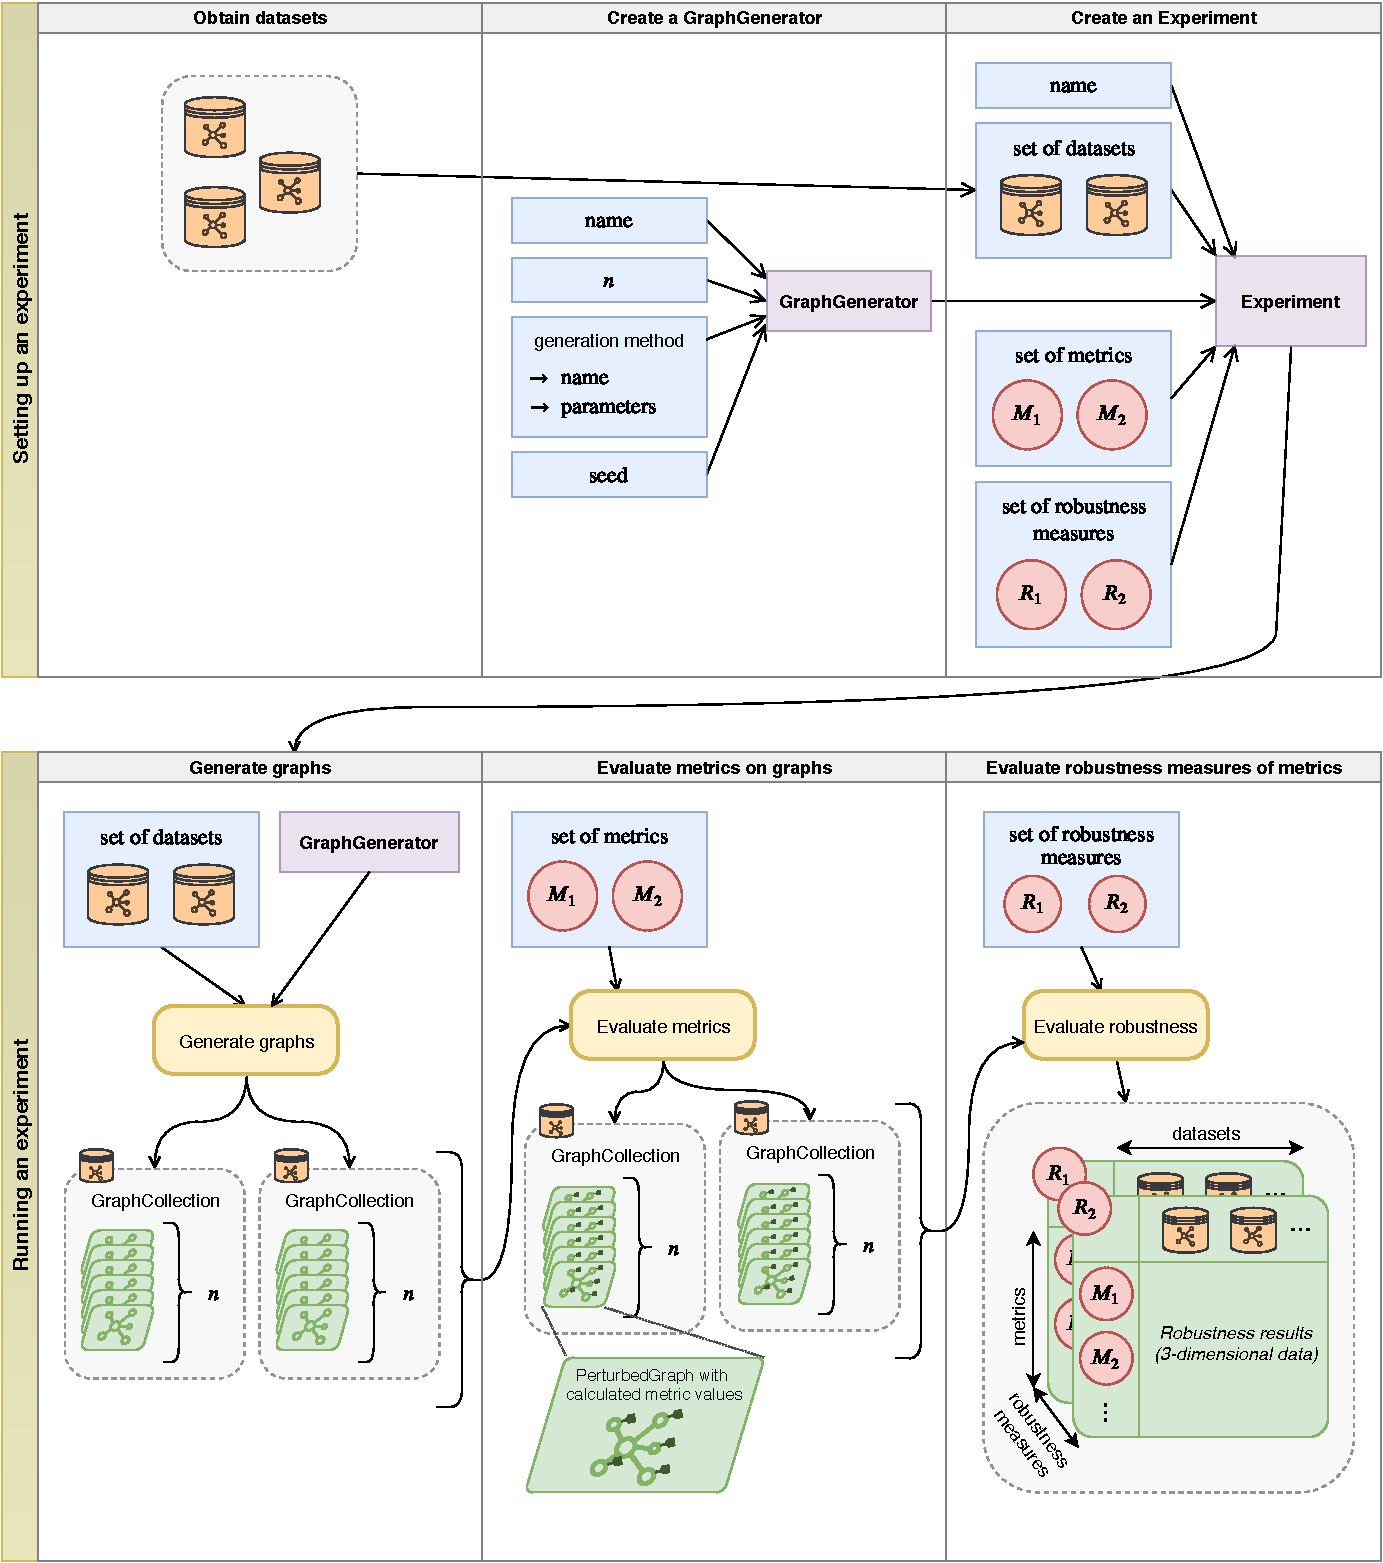
\includegraphics[width=\linewidth]{main_data_flow.pdf}
    \definecolor{diag-orange}{HTML}{D1A77D}
    \definecolor{diag-blue}{HTML}{6C8EBF}
    \definecolor{diag-violet}{HTML}{9673A6}
    \definecolor{diag-red}{HTML}{B85450}
    \definecolor{diag-yellow}{HTML}{D6B656}
    \definecolor{diag-green}{HTML}{82B366}
    \caption{Diagram showing the flow of data in individual steps of two phases: 1. setting up an experiment (the user collects/inputs data), 2. running an experiment (the program is running the computations as described in \autoref{sec:main_pipeline}). The result is a 3-dimensional data with a calculated robustness value for each from \textsl{datasets, metrics, robustness measures}.}\label{fig:main_data_flow}
    \footnotesize\justify\vspace{-0.4\baselineskip}
    Legend: \textcolor{diag-orange}{orange} -- datasets; \textcolor{diag-blue}{blue} -- user input; \textcolor{diag-violet}{violet} -- user-defined persisted entity; \textcolor{diag-red}{red} -- program-defined operations; \textcolor{diag-yellow}{yellow} -- processes; \textcolor{diag-green}{green} -- program-generated output; arrows $\rightarrow$ represent the flow of data.
\end{figure}
